
%  \section{The PSF profile analysis}

Compare to SDSS, emphasize superiority of 1 parameter vs. 6 parameters fit

Discuss profile shape stability when the seeing is rapidly  changing 

\begin{figure}
\centering
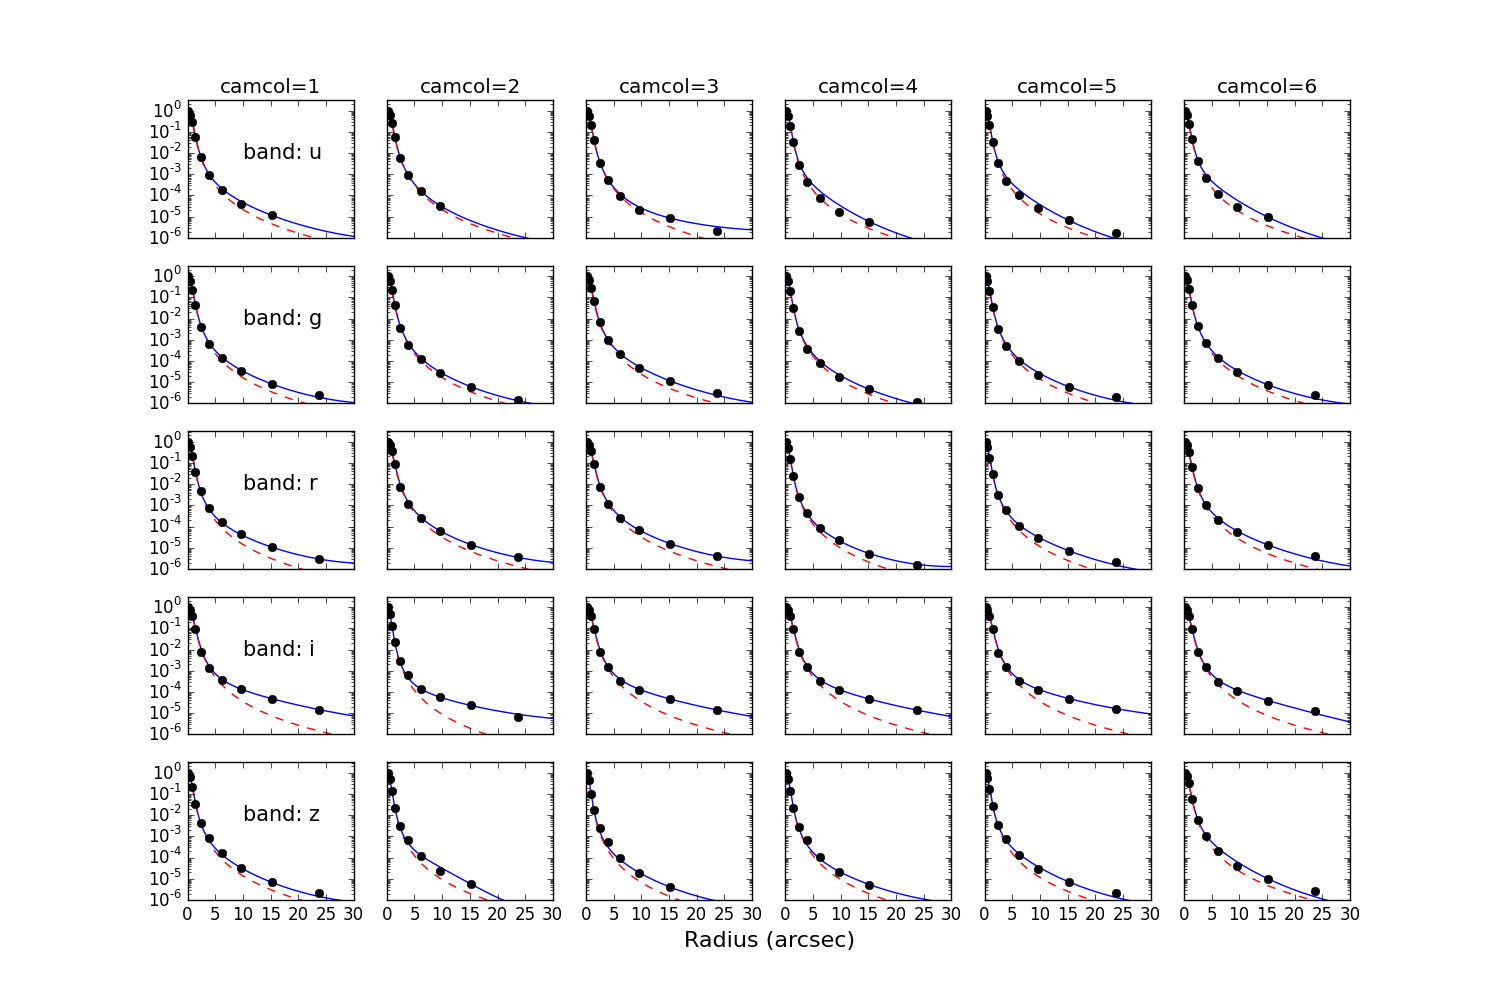
\includegraphics[width=0.9\textwidth]{FIGURES/psffit.png}
\caption{Fit to the PSF profiles from run 1033, field 200. Red curves
  are results of 1-parameter von Karman fits. Blue curves are red
  curve convolved with the instrument PSF, where the scaling factor on
  the tail component is allowed to vary.
\label{fig:psffit}}
\end{figure}
